\section{问题一的模型建立与求解}
\subsection{求解思路与模型选择}

\textbf{全时段电量流线性规划模型。}

附件1给出了同一天内的供需和电价曲线，问题一的关键在于把有限的储能用在合适的时段。若仅在电价低时充电、电价高时放电，可能过早占满午间所需的储能空间，也可能在真正的价格高峰到来前用完可放电量。因此，本文以各时段的电量分配为决策对象，将全天购电和储能变化联系起来，并与两种直观的峰谷购电策略比较，以确定问题一采用的方案。

\subsubsection{时段划分与决策变量}
将一天分为144个10分钟区间，使用第$k$段起点的采样值代表该段内的功率。相应的负载电量与光伏电量为
\begin{equation}
 E^{\mathrm L}_k=L_k\Delta t,\qquad E^{\mathrm{PV}}_k=P^{\mathrm{PV}}_k\Delta t,
 \qquad \Delta t=\frac{1}{6}\ \mathrm h.
 \label{eq:energy_conversion}
\end{equation}
例如，某段负载功率为6000 kW，该10分钟所需电量为1000 kWh。输入表中的零点虽排在末尾，但在重复代表日内对应第一段00:00--00:10；其余记录按实际时刻对应区间，而不直接以行号表示时间。

按光伏优先直接供负载的假设，先计算直供电量$m_k$、剩余负载缺口$n_k$和光伏富余$r_k$：
\begin{equation}
 \begin{aligned}
 m_k&=\min\{E^{\mathrm L}_k,E^{\mathrm{PV}}_k\},\\
 n_k&=E^{\mathrm L}_k-m_k,\qquad r_k=E^{\mathrm{PV}}_k-m_k.
 \end{aligned}
 \label{eq:pv_first}
\end{equation}
这三项均由已知数据确定。它们将同一时段分为负载需要补电或光伏存在富余两种情形，避免将本可直接使用的光伏先送入电池而产生不必要的损耗。

每段设置四个连续决策量：外网用于充电的电量$x_k$、光伏用于充电的电量$y_k$、电池向负载输出的电量$z_k$，以及段末内部储电量$S_k$。四者均以kWh计量，但前三者按设备外侧计量，$S_k$按电池内部计量。为说明购电量与这些变量的关系，将电量流向整理为图\ref{fig:energy_paths}。

\begin{inlinefigure}
 % Q1 energy-path definition: report 12.2, 15; external-side kWh.
\begin{tikzpicture}[>=Stealth, node distance=16mm, every node/.style={font=\small},
  box/.style={draw=black,rounded corners=2pt,minimum width=23mm,minimum height=10mm,align=center},
  lab/.style={fill=white,inner sep=2pt}]
\node[box] (grid) at (0,1.25) {外部电网};
\node[box] (pv) at (0,-1.25) {光伏发电};
\node[box] (battery) at (5,0) {储能设备\\$S_{k-1}\longrightarrow S_k$};
\node[box] (load) at (10,1.25) {小区负载};
\node[box] (waste) at (10,-1.25) {未利用光伏};
\draw[->] (grid.east) -- node[lab,above] {$n_k-z_k$} (load.west);
\draw[->] (grid.south east) -- node[lab,above,sloped] {$x_k$} (battery.north west);
\draw[->] (pv.north east) -- node[lab,above,sloped] {$y_k$} (battery.south west);
\draw[->] (battery.north east) -- node[lab,below,sloped] {$z_k$} (load.south west);
\draw[->] (pv.south) -- (0,-2.65) -- node[lab,below] {$m_k$：光伏直供} (11.9,-2.65) -- (11.9,1.25) -- (load.east);
\draw[->] (pv.east) -- node[lab,pos=.70,above] {$w_k=r_k-y_k$} (waste.west);
\end{tikzpicture}

 \caption{问题一的电量分配关系（各箭头表示该时段的电量）}
 \label{fig:energy_paths}
\end{inlinefigure}

图中，外网既补足电池放电后的负载缺口，也可为以后使用而充电，因此总购电量为
\begin{equation}
 q_k=n_k-z_k+x_k. \label{eq:purchase}
\end{equation}
总充电量为$E^{\mathrm{ch}}_k=x_k+y_k$，总放电量为$E^{\mathrm{dis}}_k=z_k$；未利用光伏为$w_k=r_k-y_k$。这样，购电量不再需要作为独立变量，供电和储能的每一条去向仍可单独核对。

\subsubsection{目标函数}
问题一只计普通外网购电费用。光伏为小区提供本地电源，储能损耗通过额外所需的购电量反映，不另加一笔损耗费用；题目也未给出售电收入或电池寿命成本。因此，以全天购电费用最小为目标：
\begin{equation}
 \min C=\sum_{k=1}^{144}p_kq_k
       =\sum_{k=1}^{144}p_k(n_k-z_k+x_k).
 \label{eq:objective}
\end{equation}
这里$p_k$的单位是元/kWh，$q_k$已经是10分钟电量，计算费用时不再乘$\Delta t$。目标最小化的是费用，而非购电总量；适度增加低价购电，即使带来充放电损耗，也可能减少更昂贵时段的购电支出。

\subsubsection{约束条件}
\textbf{（1）供电与光伏分配。}各时段的负载均需得到满足，充入电池的光伏不能超过该段富余，电池放电不能超过直供后的缺口：
\begin{equation}
 \begin{gathered}
 x_k\geq0,\qquad 0\leq y_k\leq r_k,\qquad 0\leq z_k\leq n_k,\\
 m_k+(q_k-x_k)+z_k=E^{\mathrm L}_k,\qquad
 m_k+y_k+w_k=E^{\mathrm{PV}}_k,\quad w_k\geq0.
 \end{gathered}
 \label{eq:balance}
\end{equation}
其中两条等式由式\eqref{eq:pv_first}和式\eqref{eq:purchase}直接保证。$q_k-x_k=n_k-z_k$为外网直接供负载的电量；允许富余光伏无法全部存入，但不给未利用电量附加售电收益。

\textbf{（2）充放电功率。}容量表示能存多少，功率表示每段能充入或放出多快。最大充电功率和放电功率均为5000 kW，故
\begin{equation}
 x_k+y_k\leq P_{\max}\Delta t,\qquad z_k\leq P_{\max}\Delta t,
 \qquad P_{\max}=5000\ \mathrm{kW}.
 \label{eq:power}
\end{equation}
每段外侧充电量或放电量因此不超过833.33 kWh。此上限约束储能设备，外网直接向负载供电的部分不占用电池充放电功率。

\textbf{（3）储电量变化及运行区间。}充电损耗发生在电量进入电池时，放电损耗发生在电量输出时，故
\begin{equation}
 S_k=S_{k-1}+\eta_{\mathrm c}(x_k+y_k)-\frac{z_k}{\eta_{\mathrm d}},
 \qquad \eta_{\mathrm c}=\eta_{\mathrm d}=0.90,
 \label{eq:soc}
\end{equation}
\begin{equation}
 1200\leq S_k\leq10800,\qquad k=1,\ldots,144.
 \label{eq:soc_bound}
\end{equation}
向设备输入100 kWh只能使内部库存增加90 kWh，而向负载输出90 kWh需要从内部扣除100 kWh。因此，外部电量经过一次完整充放后，能够用于负载的比例为$0.9\times0.9=0.81$。设备达到1200 kWh下限即不能继续放电，并不需要等到电量降至零。

\textbf{（4）日首尾电量相等。}主方案取日初储电量6000 kWh，并要求
\begin{equation}
 S_0=S_{144}=6000\ \mathrm{kWh}.
 \label{eq:cyclic}
\end{equation}
将式\eqref{eq:soc}对全天求和可得
\begin{equation}
 \sum_{k=1}^{144}z_k=\eta_{\mathrm c}\eta_{\mathrm d}
 \sum_{k=1}^{144}(x_k+y_k)=0.81\sum_{k=1}^{144}(x_k+y_k).
 \label{eq:daily_energy}
\end{equation}
这说明当天输出的储能电量需要由当天充电补回，不能依靠消耗初始库存制造低费用。6000 kWh确定主方案的比较条件，日内储电量仍可在允许区间内变化。

\subsubsection{线性结构与求解方法}
上述目标与约束均为线性关系。式\eqref{eq:pv_first}虽然含有最小值运算，但作用于已知供需数据，并未引入非线性决策。每段四个变量，共576个连续变量，144条储电递推等式将全天安排联系起来。

还需说明为何没有额外设置充电、放电的二元开关。在本问正电价、外网可直接供负载的条件下，同时充放电只会增加损耗。若某段$x_k>0$且$z_k>0$，则$n_k>0$、$r_k=0$，因而$y_k=0$。令$\delta=\min\{x_k,z_k/0.81\}>0$，将$x_k$减少$\delta$，同时将$z_k$减少$0.81\delta$，则
\begin{equation}
 \Delta S_k=-0.9\delta+\frac{0.81\delta}{0.9}=0,
 \qquad \Delta q_k=-0.19\delta<0.
 \label{eq:no_cycle}
\end{equation}
这一调整不改变储电轨迹，不破坏功率或供电约束，却严格降低费用，故同时充放不可能是最优选择。因此，本问可直接采用连续线性规划；若出现负电价或新增离散开关限制，这一结论需重新检验。

求解时，先按时间映射生成144段电量与价格，再将式\eqref{eq:objective}和式\eqref{eq:balance}--\eqref{eq:cyclic}整理成线性规划的系数矩阵与变量上下界，使用SciPy的\texttt{linprog}接口调用HiGHS。求解器以最优状态正常终止，并输出逐段购电、充放电与储电量。数值最优性及逐段约束另作独立复核，结果见本问检验部分。

\subsubsection{模型比较与方案选择}
为判断全天统一安排的实际收益，设置两种具有直观含义的参照策略。峰谷电价策略根据低价、高价门槛及目标储电量安排充放电，并考虑充放电损耗；光伏空间预留策略在相同规则上，进一步根据后续富余光伏限制提前充电，避免过早占满电池。线性规划则不预设价格门槛，而是在同一供需与设备条件下，同时确定所有时段的安排。

比较统一使用附件1的代表日、充放各90\%的效率及首尾6000 kWh条件。两种规则分别考察27组相同的参数组合：低价门槛取电价的15\%、25\%、35\%分位，高价门槛取65\%、75\%、85\%分位，目标储电量取6000、8400、10800 kWh。两者均按剩余时段的充放能力保护日末目标，恢复库存所需的实际购电全部计费，再分别取所考察组合中费用最低的结果。

峰谷电价策略、光伏空间预留策略与线性规划的全天费用依次为\RuleCost{}元、\ReserveCost{}元和\MainCost{}元。线性规划相较前两者分别节省\RuleSaving{}元和\ReserveSaving{}元，降幅为\RuleSavingPct{}\%和\ReserveSavingPct{}\%，且三种入选安排均满足逐段约束、没有未利用光伏。由此，本文选择线性规划作为问题一的购电与储能调度方案。它的优势既有实际费用比较的支持，也有在所列约束下统筹全天电量的结构依据。

光伏预留本身的作用并非在所有参数下都相同。在27组相同参数的配对中，18组费用降低、9组相同；尤其在峰谷策略费用最低的那组参数下，加入光伏预留并未改变结果。因此，预留策略各自调参后的费用较低，不能全部归因于新增预留机制。上述比较限于给定代表日和已考察的规则参数，不将规则的局部搜索结果称为该类方法的全局最优，也不据此评价未实际运行的其他算法。

\subsubsection{购电安排与结果分析}
主方案全天购电\MainPurchase{} kWh，费用\MainCost{}元，储能外侧累计充电\MainCharge{} kWh、累计放电\MainDischarge{} kWh。题目指定的六个购电区间及4小时储能汇总分别列于表\ref{tab:purchase}和表\ref{tab:storage}，其余10分钟购电结果保存在\texttt{result1.xlsx}中。

\begin{inlinetable}
 \caption{问题一指定区间的购电量及全天费用}\label{tab:purchase}
 \renewcommand{\arraystretch}{1.23}
 \begin{tabularx}{\linewidth}{l*{3}{>{\centering\arraybackslash}X}}
 \toprule
 时间段 & 10:00--10:10 & 12:00--12:10 & 14:00--14:10\\
 购电量/kWh & \BuyTen & \BuyTwelve & \BuyFourteen\\ \midrule
 时间段 & 16:00--16:10 & 18:00--18:10 & 20:00--20:10\\
 购电量/kWh & \BuySixteen & \BuyEighteen & \BuyTwenty\\ \midrule
 全天购电量/kWh & \multicolumn{3}{c}{\MainPurchase}\\
 全天购电费/元 & \multicolumn{3}{c}{\MainCost}\\
 \bottomrule
 \end{tabularx}
\end{inlinetable}

\begin{inlinetable}
 \caption{问题一各4小时区间的储能充放电量}\label{tab:storage}
 \renewcommand{\arraystretch}{1.23}
 \begin{tabularx}{\linewidth}{l*{3}{>{\centering\arraybackslash}X}}
 \toprule
 时间段 & 00:00--04:00 & 04:00--08:00 & 08:00--12:00\\
 充电量/kWh & \ChargeA & \ChargeB & \ChargeC\\
 放电量/kWh & \DischargeA & \DischargeB & \DischargeC\\ \midrule
 时间段 & 12:00--16:00 & 16:00--20:00 & 20:00--24:00\\
 充电量/kWh & \ChargeD & \ChargeE & \ChargeF\\
 放电量/kWh & \DischargeD & \DischargeE & \DischargeF\\ \midrule
 零点储电量/kWh & \multicolumn{3}{c}{6000.00}\\
 24点储电量/kWh & \multicolumn{3}{c}{6000.00}\\
 \bottomrule
 \end{tabularx}
\end{inlinetable}

4小时内同时出现充电量和放电量，表示这些动作发生在其中不同的10分钟区间；逐段结果没有同时充放电。全天累计充电量超过设备容量也不矛盾，因为电池在一天内可以反复使用，容量限制的是某一时刻的库存。

线性规划在凌晨补充电量，在早间用电阶段释放一部分库存，并利用午间富余光伏和适当的外网充电为晚间作准备。到16点，电池储电量达到10800 kWh。晚间虽已进入较高电价区间，方案仍保留一部分电量等待更贵的时段：20点尚有\EveningState{} kWh，而两种规则策略均已降至1200 kWh下限。20:40--20:50电价达到1.3952元/kWh时，线性规划由电池补足负载缺口，该段外网购电为零；两种规则则仍需购买\PeakRulePurchase{} kWh。日末价格回落后，方案再补回6000 kWh的起始库存。

节费并非来自减少所有购电。相较峰谷规则，线性规划多购电\ExtraPurchase{} kWh，恰好对应更多充放电带来的额外损耗；三种入选策略均已利用全部富余光伏，光伏利用率也不是这里费用差异的来源。真正的收益在于以更多低价电替代高价电。以外网充电为例，在低价$p_a$时购买1 kWh，经充放后只能替代高价$p_b$时的0.81 kWh，只有$p_a<0.81p_b$才具有基本价格收益；实际能转移多少，还受容量、功率和后续供需共同限制。

上述购电与储能变化可结合图\ref{fig:dispatch}理解。图中将三种策略的电价、储电量和购电功率放在同一时间轴上。上图帮助定位高价时段，中图说明电量何时留存、何时使用，下图给出相应的外网购电变化。

\begin{inlinefigure}
 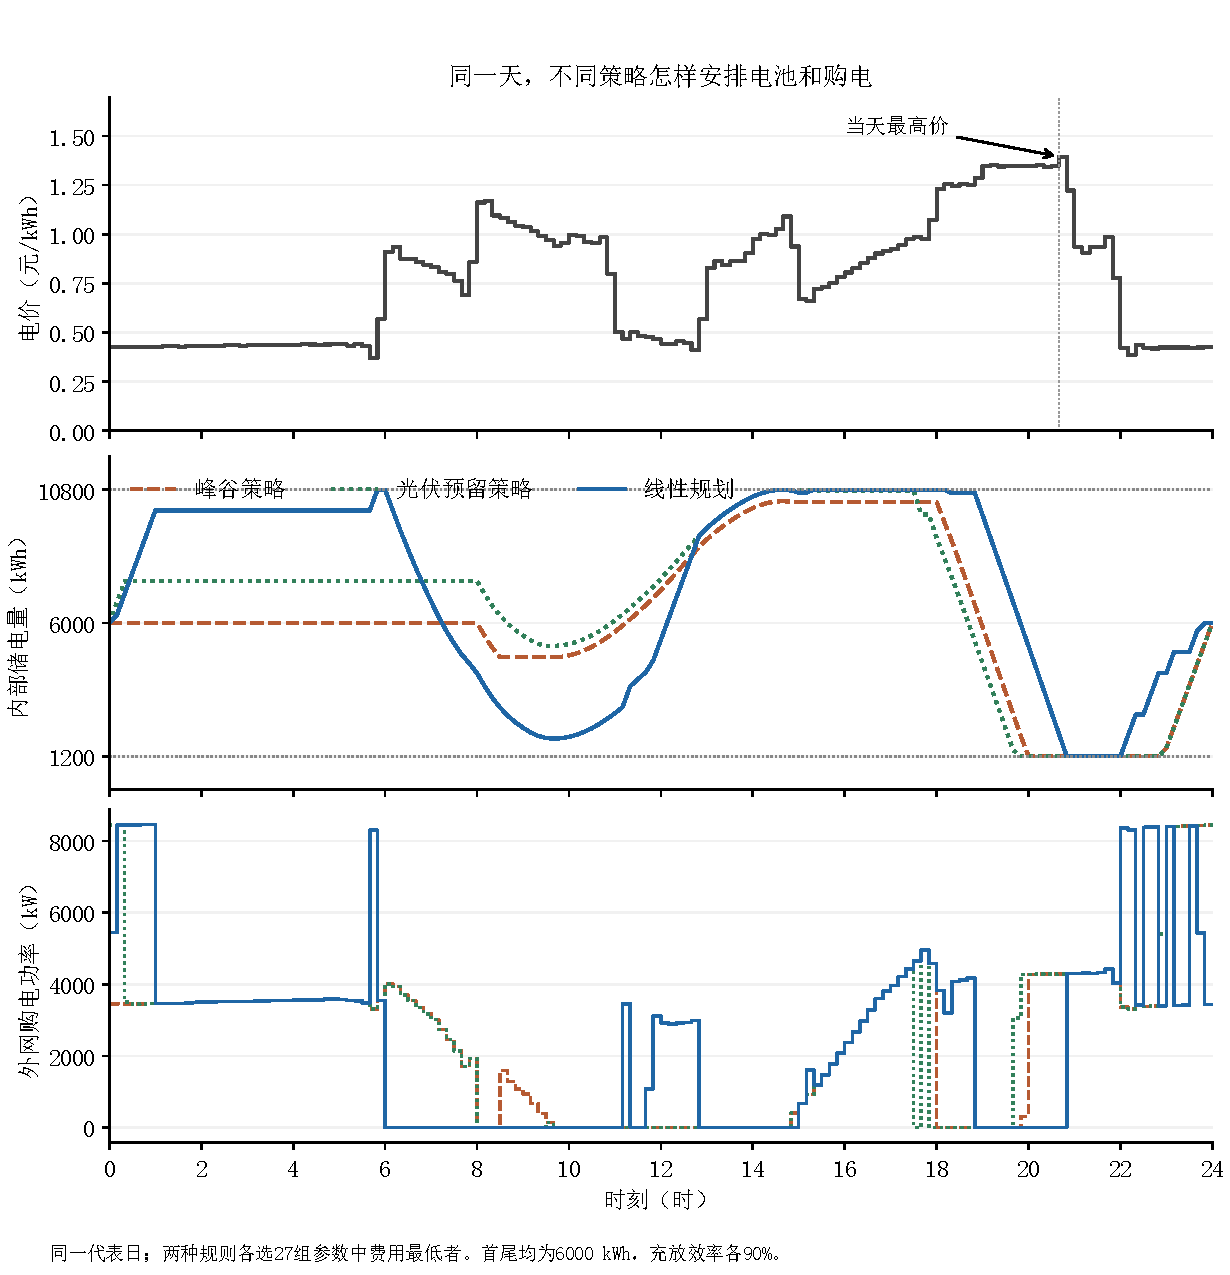
\includegraphics[width=0.90\linewidth]{q1_daily_dispatch.pdf}
 \caption{三种策略在相同代表日下的购电与储能安排}
 \label{fig:dispatch}
\end{inlinefigure}

\subsubsection{模型检验与初始储电量敏感性分析}
首先按导出的10分钟结果独立复算供需平衡、储电递推、容量与功率上限及全天费用，并核对首尾电量。三个起点案例的最大储电递推残差约为$1.34\times10^{-12}$ kWh；由求解器对偶信息独立重算的费用下界与实际可行方案费用之差最大约为$1.22\times10^{-12}$元。可行费用与下界在数值精度内一致，支持所列线性规划的最优性判断。此外，通过同价充放无套利、低高价两段充放以及初始库存不能免费消耗的小例子核对损耗与边界表达，并将导出表按真实时间逐项对应，避免零点置末造成结果错位。

问题一要求首尾电量相同，但相同的起点数值仍可能影响当天安排。为考察这种影响，保持供需、电价、效率和设备条件不变，分别以1200、6000和10800 kWh开始，每种情况均重新优化，并在日末恢复到各自起点。所得费用分别为\LowInitialCost{}元、\MainCost{}元和\HighInitialCost{}元；相较6000 kWh主方案，两个边界起点分别增加\LowInitialDelta{}元和\HighInitialDelta{}元，增幅为\LowInitialPct{}\%和\HighInitialPct{}\%。

三个案例的全天购电、累计充放电和光伏利用量相同，20点也都保留约\EveningState{} kWh，并避开最高价区间购电。但费用接近不表示逐段安排不变：两个替代起点各有14段购电量改变，均将5333.33 kWh从一部分时段转移到另一部分时段。低起点少了4800 kWh内部库存，凌晨需要多买$4800/0.9=5333.33$ kWh补充，日末则相应少补；高起点虽能减少凌晨补电，却必须在日末恢复更多库存。受充电功率和剩余时间限制，高起点还需在21:50--22:00以0.7764元/kWh额外购买666.67 kWh，因而开始时电量更多并不保证全天费用更低。

这三个已检验起点下，重新安排后的费用差异均不到1\%，且为晚间高价时段留电的特征保持一致；初始电量主要改变凌晨与日末的补电分配。检验只覆盖这三个取值，不能据此认定6000 kWh是整个允许区间内的最佳起点，也不能将重新优化后的结果解释为固定计划能够抵抗供需预测误差。问题一给出的是已知代表日下的调度依据；实际供需偏差出现后，计划与执行之间的差异还需在后续问题中处理。
